\chapter{酸碱平衡与优势反应法}\label{ch:b1:predominant-reaction}

醋能溶解水壶中的水垢，柠檬汁亦然，且稍快一些。
无论吃进什么，血液的 pH 总保持在狭窄的范围内；碳酸饮料呈酸性，
是因为其中溶有二氧化碳。这些
现象都属于水中的酸碱平衡。化学家面对含有多种酸、碱的溶液，
如混合物、\omterm{def:b1:predominant-reaction:buffer}{缓冲溶液}或\omterm{def:b1:predominant-reaction:polyprotic}{多元酸}——
需要一种可靠的方法，求出其 pH 与各物种的浓度。
本章建立这一方法：一套强度标度、\omterm{def:b1:predominant-reaction:predominance}{优势区域图}，
以及\emph{\omterm{def:b1:predominant-reaction:predominant-reaction}{优势反应}
法}，它可将任意混合体系归结为唯一起决定作用的那一个反应。

\begin{recall}
第 1 册（十二年级）中已定义\omterm{def:b1:predominant-reaction:bronsted}{布朗斯特酸}与碱、
\omterm{def:b1:predominant-reaction:acidity-constant}{酸度常数} $K_a$ 与 $\mathrm{p}K_a$、\omterm{def:b1:predominant-reaction:autoprotolysis}{水的离子积}，以及\omterm{def:b1:predominant-reaction:strong-acid}{强酸}、
\omterm{def:b1:predominant-reaction:strong-acid}{强碱}的 pH，并画出了\omterm{def:b1:predominant-reaction:predominance}{优势区域图}。\omterm{def:b1:extent-q-and-k:quotient}{反应商}、
平衡常数，以及溶质（$c/c^\circ$）和
溶剂（1）的\omterm{def:b1:extent-q-and-k:activity}{活度}，均已在\cref{ch:b1:extent-q-and-k}中定义；
本章中，$c^\circ = \qty{1}{mol/L}$ 不再写入商中。
\end{recall}

\begin{omfigure}
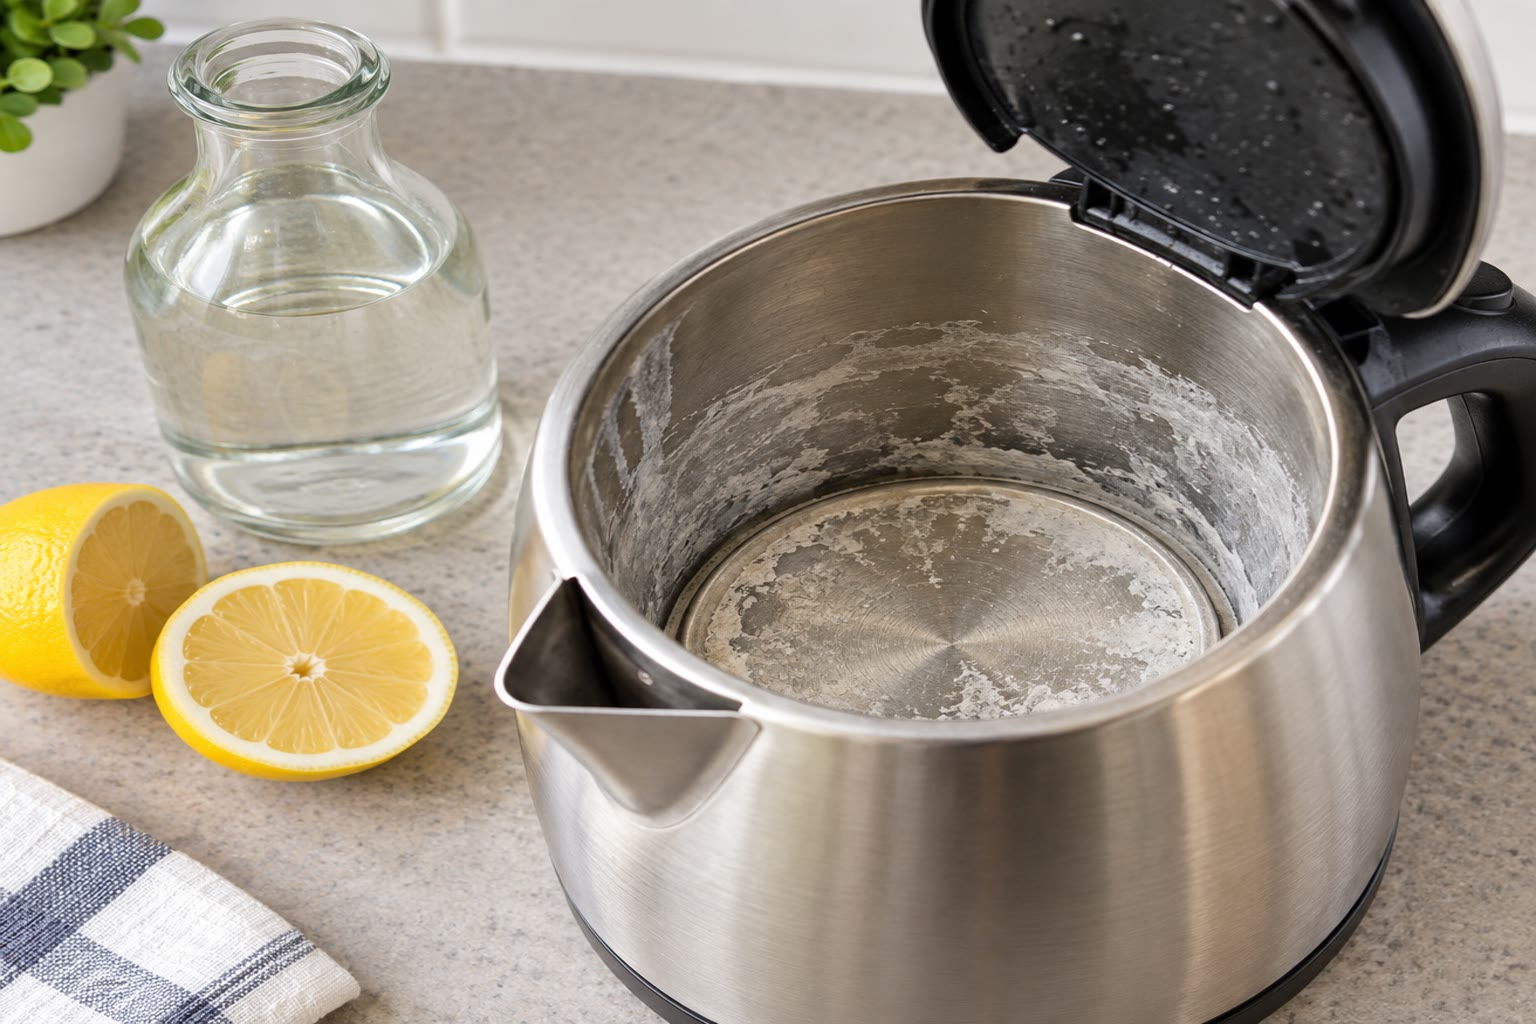
\includegraphics[width=0.5\linewidth]{images/book2/ai/b1-10-descaling.jpg}

{\small 水壶中的水垢，即碳酸钙。醋和柠檬汁中的\omterm{def:b1:predominant-reaction:strong-acid}{弱酸}
与碳酸根离子反应，使其溶解。}
\end{omfigure}

\section{布朗斯特共轭对与 pH}

\begin{definition}[布朗斯特酸、碱与共轭对]\label{def:b1:predominant-reaction:bronsted}
称\emph{布朗斯特酸}\index{布朗斯特酸}为能给出一个
质子 \ce{H+} 的物种；称\emph{布朗斯特碱}\index{布朗斯特碱}为能接受一个
质子的物种。酸 HA 失去一个质子后所成的碱 A，与之构成
\emph{酸碱共轭对}\index{酸碱共轭对} HA/A，二者由形式半反应式
$\mathrm{HA} \rightleftharpoons
\mathrm{A} + \ce{H+}$ 相联系。在水中，质子从不以游离形式存在，而是
由水分子以 \ce{H3O+} 的形式携带。
\end{definition}

\begin{definition}[两性物质]\label{def:b1:predominant-reaction:ampholyte}
称\emph{两性物质}\index{两性物质}既是一个共轭对的碱，又是另一个共轭对的酸：
水（\ce{H3O+}/\ce{H2O} 与 \ce{H2O}/\ce{OH-}）、
碳酸氢根离子（\ce{CO2,H2O}/\ce{HCO3-} 与 \ce{HCO3-}/\ce{CO3^{2-}}）、
磷酸二氢根离子。
\end{definition}

\begin{definition}[自耦电离、离子积、pH]\label{def:b1:predominant-reaction:autoprotolysis}
水发生\emph{自耦电离}\index{自耦电离}，
\ce{2H2O <=> H3O+ + OH-}，其 $K_e = [\ce{H3O+}][\ce{OH-}]$ 为常数，称为
\emph{水的离子积}\index{水的离子积}；在
\qty{25}{\celsius} 时，$K_e = 10^{-14.00}$，故 $\mathrm{p}K_e = 14.00$。溶液的 pH
定义为 $\mathrm{pH} = -\log a(\ce{H3O+}) \approx -\log[\ce{H3O+}]$。
溶液呈中性，当 $[\ce{H3O+}] = [\ce{OH-}]$ 时，
即 \qty{25}{\celsius} 下 $\mathrm{pH} = \mathrm{p}K_e/2 = 7.00$。
% ledger: dfg:H2O_l, dfg:OH-_ao (pKe computed in figdata/bachelor-1/aqueous-constants.py)
\end{definition}

\section{强度：\texorpdfstring{$K_a$}{Ka}、\texorpdfstring{p$K_a$}{pKa}与拉平效应}

\begin{definition}[酸度常数]\label{def:b1:predominant-reaction:acidity-constant}
共轭对 HA/A 的\emph{酸度常数}\index{酸度常数}
是酸与水反应的平衡常数，
\[
  \mathrm{HA} + \ce{H2O} \rightleftharpoons \mathrm{A} + \ce{H3O+}, \qquad
  K_a = \frac{[\mathrm{A}][\ce{H3O+}]}{[\mathrm{HA}]}, \qquad
  \mathrm{p}K_a = -\log K_a .
\]
$K_a$ 越大（$\mathrm{p}K_a$ 越小），则酸越强，
而其共轭碱越弱。
\end{definition}

\begin{definition}[强酸与弱酸、强碱与弱碱]\label{def:b1:predominant-reaction:strong-acid}
酸在水中，若与水的反应进行完全，则称为\emph{强酸}\index{强酸}
（即溶液中不再残留 HA 分子，如盐酸、硝酸、高氯酸及硫酸的第一步电离）；
否则称为\emph{弱酸}\index{弱酸}。碱在水中，
若与水的反应进行完全并生成 \ce{OH-}，则称为\emph{强碱}\index{强碱}
（如氢氧化物、氧离子、醇盐）；
否则称为\emph{弱碱}\index{弱碱}。
\end{definition}

\begin{definition}[拉平效应]\label{def:b1:predominant-reaction:levelling}
在水中，凡强于 \ce{H3O+} 的酸，皆完全反应生成
\ce{H3O+}；凡强于 \ce{OH-} 的碱，皆完全反应生成
\ce{OH-}，二者强度无从区分。这就是
溶剂的\emph{拉平效应}\index{拉平效应}。水中的\omterm{def:b1:predominant-reaction:strong-acid}{弱酸}
与\omterm{def:b1:predominant-reaction:strong-acid}{弱碱}的 $0 < \mathrm{p}K_a < 14$，而水本身的共轭对
（$\mathrm{p}K_a(\ce{H3O+}/\ce{H2O}) = 0$ 与
$\mathrm{p}K_a(\ce{H2O}/\ce{OH-}) = 14$）界定了这一标度的两端。
\end{definition}

\begin{center}
\small
\begin{tabular}{lll@{\hspace{2.5em}}lll}
\hline
共轭对 & p$K_a$ & & 共轭对 & p$K_a$ & \\
\hline
\ce{HSO4-}/\ce{SO4^{2-}} & 1.99 & & \ce{CO2,H2O}/\ce{HCO3-} & 6.37 & \\
\ce{H3PO4}/\ce{H2PO4-} & 2.15 & & \ce{H2PO4-}/\ce{HPO4^{2-}} & 7.21 & \\
\ce{HF}/\ce{F-} & 3.16 & & \ce{HClO}/\ce{ClO-} & 7.55 & \\
\ce{HCOOH}/\ce{HCOO-} & 3.74 & & \ce{NH4+}/\ce{NH3} & 9.25 & \\
\ce{CH3COOH}/\ce{CH3COO-} & 4.76 & & \ce{C6H5OH}/\ce{C6H5O-} & 9.99 & \\
\ce{C6H5NH3+}/\ce{C6H5NH2} & 4.60 & & \ce{HCO3-}/\ce{CO3^{2-}} & 10.33 & \\
\ce{C6H5COOH}/\ce{C6H5COO-} & 4.21 & & \ce{CH3NH3+}/\ce{CH3NH2} & 10.66 & \\
\hline
\end{tabular}
\end{center}
% ledger: pka:methanoic, pka:ethanoic, pka:anilinium, pka:benzoic,
% pka:phenol, pka:methylammonium (IUPAC dataset); dfg:HSO4-_ao,
% dfg:SO42-_ao, dfg:H3PO4_ao, dfg:H2PO4-_ao, dfg:HPO42-_ao, dfg:HF_ao,
% dfg:F-_ao, dfg:CO2_ao, dfg:HCO3-_ao, dfg:CO32-_ao, dfg:HClO_ao,
% dfg:ClO-_ao, dfg:NH4+_ao, dfg:NH3_ao (pKa computed from NBS-82)

\section{优势区域图与分布图}

\begin{definition}[优势区域图与分布图]\label{def:b1:predominant-reaction:predominance}
对于\omterm{def:b1:predominant-reaction:bronsted}{酸碱共轭对} HA/A，$\mathrm{pH} = \mathrm{p}K_a + \log([\mathrm{A}]/[\mathrm{HA}])$：
酸占优势（$[\mathrm{HA}] > [\mathrm{A}]$）的区间为
$\mathrm{pH} < \mathrm{p}K_a$，碱占优势的区间为 $\mathrm{pH} > \mathrm{p}K_a$。
\emph{优势区域图}\index{优势区域图}是将 pH 轴
在各 $\mathrm{p}K_a$ 处分割成各形态占优势的区域。
\emph{分布图}\index{分布图}
给出各形态所占分数 $[\text{形态}]/C$，随 pH 而变。
\end{definition}

\begin{proposition}[亨德森关系与分数]\label{prop:b1:predominant-reaction:henderson}
设\omterm{def:b1:predominant-reaction:bronsted}{酸碱共轭对} HA/A 的总浓度为 $C = [\mathrm{HA}] + [\mathrm{A}]$，
\[
  \mathrm{pH} = \mathrm{p}K_a + \log\frac{[\mathrm{A}]}{[\mathrm{HA}]}, \qquad
  \frac{[\mathrm{HA}]}{C} = \frac{1}{1 + 10^{\mathrm{pH} - \mathrm{p}K_a}}, \qquad
  \frac{[\mathrm{A}]}{C} = \frac{1}{1 + 10^{\mathrm{p}K_a - \mathrm{pH}}} .
\]
当 pH 与 $\mathrm{p}K_a$ 相差一个单位时，次要形态的占比低于
总量的 10\,\%；相差两个单位时，低于 1\,\%。
\end{proposition}

\begin{proof}
对 $K_a = [\mathrm{A}][\ce{H3O+}]/[\mathrm{HA}]$ 取对数，于是
即 $[\mathrm{A}]/[\mathrm{HA}] = 10^{\mathrm{pH}-\mathrm{p}K_a}$，再将
$[\mathrm{HA}]$ 除以 $[\mathrm{HA}] + [\mathrm{A}]$ 即得分数。
当 $\mathrm{pH} = \mathrm{p}K_a + 1$ 时，$[\mathrm{HA}]/C = 1/11 < 10\,\%$；
当 $+2$ 时，为 $1/101$。
\end{proof}

\begin{omfigure}
\begin{tikzpicture}
\begin{axis}[name=e,
  width=0.48\linewidth, height=5.2cm, xmin=0, xmax=14, ymin=0, ymax=1.05,
  axis x line=bottom, axis y line=left, xlabel={pH}, ylabel={分数},
  xtick={0,2,4,6,8,10,12,14},
  tick label style={font=\small}, label style={font=\small}]
\addplot[omDef, thick] table[x=pH, y=HA] {figdata/out/bachelor-1-distribution-diagrams-ethanoic.dat};
\addplot[omThm, thick] table[x=pH, y=A] {figdata/out/bachelor-1-distribution-diagrams-ethanoic.dat};
\draw[dotted] (axis cs:4.76,0) -- (axis cs:4.76,0.5);
\node[omDef, font=\footnotesize, anchor=west] at (axis cs:0.3,0.3) {\ce{CH3COOH}};
\node[omThm, font=\footnotesize, anchor=east] at (axis cs:13.7,0.3) {\ce{CH3COO-}};
\node[font=\small, anchor=north west] at (axis cs:4.8,0.48) {4.76};
\end{axis}
\begin{axis}[at={(e.east)}, anchor=west, xshift=1.1cm,
  width=0.48\linewidth, height=5.2cm, xmin=0, xmax=14, ymin=0, ymax=1.05,
  axis x line=bottom, axis y line=left, xlabel={pH}, ylabel={分数},
  xtick={0,2,4,6,8,10,12,14},
  legend style={font=\scriptsize, draw=none, at={(0.5,1.04)}, anchor=south, legend columns=4},
  tick label style={font=\small}, label style={font=\small}]
\addplot[omDef, thick] table[x=pH, y=H3A] {figdata/out/bachelor-1-distribution-diagrams-phosphoric.dat};
\addplot[omMeth, thick] table[x=pH, y=H2A] {figdata/out/bachelor-1-distribution-diagrams-phosphoric.dat};
\addplot[omProp, thick] table[x=pH, y=HA] {figdata/out/bachelor-1-distribution-diagrams-phosphoric.dat};
\addplot[omThm, thick] table[x=pH, y=A] {figdata/out/bachelor-1-distribution-diagrams-phosphoric.dat};
\legend{\ce{H3PO4}, \ce{H2PO4-}, \ce{HPO4^{2-}}, \ce{PO4^{3-}}}

\end{axis}
\end{tikzpicture}

\begin{tikzpicture}[font=\small, >={Stealth}]
  \draw[->, thick] (0,0) -- (14.2*0.85,0) node[right] {pH};
  \foreach \x/\l in {2.15/2.15, 7.21/7.21, 12.34/12.34}
    \draw (\x*0.85,0.15) -- (\x*0.85,-0.15) node[below] {\l};
  \node[above] at (1.07*0.85,0.1) {\ce{H3PO4}};
  \node[above] at (4.68*0.85,0.1) {\ce{H2PO4-}};
  \node[above] at (9.78*0.85,0.1) {\ce{HPO4^{2-}}};
  \node[above] at (13.3*0.85,0.1) {\ce{PO4^{3-}}};
\end{tikzpicture}

{\small 乙酸（左）与磷酸
（右）的\omterm{def:b1:predominant-reaction:predominance}{分布图}，以及磷酸的\omterm{def:b1:predominant-reaction:predominance}{优势区域图}。每两条相邻曲线的
交点位于某个 $\mathrm{p}K_a$ 处；\omterm{def:b1:predominant-reaction:ampholyte}{两性物质}
\ce{H2PO4-} 与 \ce{HPO4^{2-}} 在各自区域中部几乎只以
一种形态存在。}
\end{omfigure}

\section{优势反应法}

\begin{proposition}[酸碱反应的常数]\label{prop:b1:predominant-reaction:k-of-reaction}
\omterm{def:b1:predominant-reaction:bronsted}{酸碱共轭对}中的酸 $\mathrm{HA}_1$ 与另一共轭对中的碱
$\mathrm{A}_2$ 的反应，
$\mathrm{HA}_1 + \mathrm{A}_2 \rightleftharpoons \mathrm{A}_1 + \mathrm{HA}_2$,
其常数为
\[
  K = \frac{K_{a1}}{K_{a2}} = 10^{\,\mathrm{p}K_{a2} - \mathrm{p}K_{a1}} .
\]
反应有利（$K > 1$），条件是所给的酸
比其所生成的酸更强（$\mathrm{p}K_{a1} < \mathrm{p}K_{a2}$）；当
按\cref{met:b1:extent-q-and-k:quantitative}的意义，反应为\omterm{def:b1:extent-q-and-k:quantitative}{定量反应}，
当 $\mathrm{p}K_a$ 之差超过约 4 时。
\end{proposition}

\begin{proof}
该反应是 $\mathrm{HA}_1 + \ce{H2O} \rightleftharpoons
\mathrm{A}_1 + \ce{H3O+}$（$K_{a1}$）与 $\mathrm{HA}_2 +
\ce{H2O} \rightleftharpoons \mathrm{A}_2 + \ce{H3O+}$ 的逆反应（$1/K_{a2}$）之和；
由\cref{prop:b1:extent-q-and-k:combine-k}可得 $K = K_{a1}/K_{a2}$。
\end{proof}

\begin{definition}[优势反应与等效溶液]\label{def:b1:predominant-reaction:predominant-reaction}
在含有多种酸和碱的溶液中，
\emph{优势反应}\index{优势反应}是平衡常数最大的反应，
即溶液中存在的最\omterm{def:b1:predominant-reaction:strong-acid}{强酸}与最\omterm{def:b1:predominant-reaction:strong-acid}{强碱}之间的反应。若其为
\omterm{def:b1:extent-q-and-k:quantitative}{定量反应}，则将其视为完全进行，并以
\emph{等效溶液}\index{等效溶液}代替原溶液：即该反应完成后
所得的溶液，其 pH 与
原溶液相同。
\end{definition}

\begin{method}[主反应方法]\label{met:b1:predominant-reaction:method}
求溶液的 pH 与组成：
\begin{enumerate}
  \item 列出所引入的物种（包括水），并将其\omterm{def:b1:predominant-reaction:bronsted}{酸碱共轭对}
        置于 $\mathrm{p}K_a$ 标度上，酸在一侧，碱在另一侧；
  \item 找出存在的最\omterm{def:b1:predominant-reaction:strong-acid}{强酸}和最\omterm{def:b1:predominant-reaction:strong-acid}{强碱}；
  \item 若两者反应的常数较大（$K > 10^4$，或
        $\Delta\mathrm{p}K_a > 4$），则将该反应视为完全进行，并写出
        \omterm{def:b1:predominant-reaction:predominant-reaction}{等效溶液}；返回第 2 步；
  \item 当主反应的常数较小时，它决定溶液
        的 pH：写出其进度表并解 $Q = K$，通常采用
        其\omterm{def:b1:extent-q-and-k:extent}{反应进度}较小的假设；
  \item 检验假设：次要物种确实很少，并且
        其他反应（包括水的\omterm{def:b1:predominant-reaction:autoprotolysis}{自耦电离}）均可
        忽略。
\end{enumerate}
\end{method}

\begin{omfigure}
\begin{tikzpicture}[font=\small, >={Stealth}]
  \draw[->, thick] (0,-0.3) -- (0,7.6) node[above] {p$K_a$};
  \foreach \y/\a/\b in {0/\ce{H3O+}/\ce{H2O}, 1.58/\ce{HF}/\ce{F-}, 2.38/\ce{CH3COOH}/\ce{CH3COO-},
      3.62/\ce{H2PO4-}/\ce{HPO4^{2-}}, 4.62/\ce{NH4+}/\ce{NH3}, 7/\ce{H2O}/\ce{OH-}} {
    \draw (-0.12,\y) -- (0.12,\y);
    \node[anchor=east] at (-0.2,\y) {\a};
    \node[anchor=west] at (0.2,\y) {\b};
  }
  \foreach \y/\l in {0/0, 1.58/3.16, 2.38/4.76, 3.62/7.21, 4.62/9.25, 7/14} \node[black!60, anchor=west] at (3.0,\y) {\l};
  \draw[->, omThm, thick] (-1.6,2.55) -- (1.2,4.45);
  \node[omThm, anchor=west, align=left] at (4.2,3.5) {酸与其上方的任一 \\碱发生反应：$K > 1$};
  \node[anchor=south] at (-1.4,7.35) {酸};
  \node[anchor=south] at (1.2,7.35) {碱};
\end{tikzpicture}

{\small $\mathrm{p}K_a$ 标度（图中 p$K_a$ 向上递增，
数值标在右侧）。酸易与标度上位于其上方的任一碱发生反应：
此处为乙酸与氨，
$K = 10^{9.25 - 4.76} = 10^{4.49}$。}
\end{omfigure}

\begin{proposition}[简单溶液的 pH]\label{prop:b1:predominant-reaction:ph-formulas}
浓度为 $C$（单位 \unit{mol/L}），记 $\mathrm{p}C = -\log C$：
\begin{itemize}
  \item \omterm{def:b1:predominant-reaction:strong-acid}{强酸}：$\mathrm{pH} = \mathrm{p}C$，适用于
        $\mathrm{pH} < 6.5$；
  \item \omterm{def:b1:predominant-reaction:strong-acid}{弱酸}，解离很少：$\mathrm{pH} = \frac12(\mathrm{p}K_a
        + \mathrm{p}C)$，若 $\mathrm{pH} < \mathrm{p}K_a - 1$；
  \item \omterm{def:b1:predominant-reaction:strong-acid}{弱碱}，质子化很少：$\mathrm{pH} = \frac12(\mathrm{p}K_e +
        \mathrm{p}K_a - \mathrm{p}C)$，若 $\mathrm{pH} > \mathrm{p}K_a +
        1$；
  \item \omterm{def:b1:predominant-reaction:ampholyte}{两性物质}，且 $\mathrm{p}K_{a2} - \mathrm{p}K_{a1} > 4$：
        $\mathrm{pH} = \frac12(\mathrm{p}K_{a1} + \mathrm{p}K_{a2})$，
        无论 $C$ 为何值（若溶液不太稀）。
\end{itemize}
\end{proposition}

\begin{proof}
\omterm{def:b1:predominant-reaction:strong-acid}{强酸}：\ce{HA + H2O -> A- + H3O+} 完全进行，$[\ce{H3O+}] = C$，
水自身的贡献（$10^{-7}$）在 $C > 10^{-6.5}$ 时可忽略。
\omterm{def:b1:predominant-reaction:strong-acid}{弱酸}：主反应为 $\mathrm{HA} + \ce{H2O}
\rightleftharpoons \mathrm{A} + \ce{H3O+}$，\omterm{def:b1:extent-q-and-k:extent}{反应进度} $x = [\ce{H3O+}]
= [\mathrm{A}]$；若 $x \ll C$，则 $K_a = x^2/C$，$\mathrm{pH} = \frac12(\mathrm{p}K_a
+ \mathrm{p}C)$；假设 $[\mathrm{A}] < [\mathrm{HA}]/10$
等价于 $\mathrm{pH} < \mathrm{p}K_a - 1$。\omterm{def:b1:predominant-reaction:strong-acid}{弱碱}的情形与此相同，反应为 $\mathrm{A} +
\ce{H2O} \rightleftharpoons \mathrm{HA} + \ce{OH-}$，常数为 $K_e/K_a$。
\omterm{def:b1:predominant-reaction:ampholyte}{两性物质} HA$^-$：主反应为 $2\,\mathrm{HA}^- \rightleftharpoons
\mathrm{H_2A} + \mathrm{A}^{2-}$，故 $[\mathrm{H_2A}] = [\mathrm{A}^{2-}]$；
将 $K_{a1} = [\mathrm{HA}^-]h/[\mathrm{H_2A}]$ 与 $K_{a2} =
[\mathrm{A}^{2-}]h/[\mathrm{HA}^-]$ 相乘，得 $h^2 = K_{a1}K_{a2}$。
\end{proof}

\begin{omfigure}
\begin{tikzpicture}
\begin{axis}[
  width=0.66\linewidth, height=5.6cm, xmin=0, xmax=8, ymin=0, ymax=8,
  axis x line=bottom, axis y line=left,
  xlabel={$\mathrm{p}C = -\log C$}, ylabel={pH},
  xtick={0,1,2,3,4,5,6,7,8}, ytick={0,1,2,3,4,5,6,7,8},
  tick label style={font=\small}, label style={font=\small},
  legend style={font=\small, draw=none, at={(0.02,0.98)}, anchor=north west}]
\addplot[omDef, very thick] table[x=pC, y=pH] {figdata/out/bachelor-1-weak-acid-ph.dat};
\addplot[omProp, dashed] table[x=pC, y=weak] {figdata/out/bachelor-1-weak-acid-ph.dat};
\addplot[black!50, dotted, thick] table[x=pC, y=strong] {figdata/out/bachelor-1-weak-acid-ph.dat};
\draw[black!30] (axis cs:0,7) -- (axis cs:8,7);
\legend{精确, $\frac12(\mathrm{p}K_a + \mathrm{p}C)$, $\mathrm{pH} = \mathrm{p}C$}
\end{axis}
\end{tikzpicture}

{\small 乙酸溶液的 pH 随 $\mathrm{p}C$ 变化，
由电荷平衡精确算得。浓度较高时，酸解离很少，
遵循 $\frac12(\mathrm{p}K_a + \mathrm{p}C)$；若稀释至
约 $10^{-6}$ mol/L 以下，则酸完全解离，表现为
\omterm{def:b1:predominant-reaction:strong-acid}{强酸}；极稀时，pH 趋于 7。}
\end{omfigure}

\begin{example}[乙酸与氨]\label{ex:b1:predominant-reaction:mixture}
将 \qty{0.10}{mol} 乙酸与 \qty{0.10}{mol} 氨
在 \qty{1.0}{L} 中混合。最\omterm{def:b1:predominant-reaction:strong-acid}{强酸}为 \ce{CH3COOH}，
最\omterm{def:b1:predominant-reaction:strong-acid}{强碱}为 \ce{NH3}：\ce{CH3COOH + NH3 <=> CH3COO- + NH4+}，$K = 10^{9.25 - 4.76} =
10^{4.49}$，该反应为\omterm{def:b1:extent-q-and-k:quantitative}{定量反应}。\omterm{def:b1:predominant-reaction:predominant-reaction}{等效溶液}中
含 \qty{0.10}{mol/L} 的 \ce{CH3COO-} 和 \ce{NH4+}。
其主反应 \ce{NH4+ + CH3COO- <=> NH3 + CH3COOH}，常数较小，
为 $10^{-4.49}$，并保持 $[\ce{NH3}] = [\ce{CH3COOH}]$，于是类似于\omterm{def:b1:predominant-reaction:ampholyte}{两性物质}，
$\mathrm{pH} = \frac12(4.76 + 9.25) = 7.01$。
\end{example}

\section{多元酸与缓冲溶液}

\begin{definition}[多元酸]\label{def:b1:predominant-reaction:polyprotic}
能依次给出多个质子的酸称为\emph{多元酸}\index{多元酸}，
每一步各有其自身的常数：磷酸 \ce{H3PO4}
（$\mathrm{p}K_a$ = 2.15、7.21、12.34），碳酸
（\ce{CO2,H2O}；6.37、10.33），硫酸（一级酸性强，
二级 1.99）。逐级的 $\mathrm{p}K_a$ 依次增大：从一个已带负电的
物种上移去质子所需代价更大。
\end{definition}

\begin{example}[\texorpdfstring{\qty{0.10}{mol/L}}{0.10 mol/L}下的磷酸]\label{ex:b1:predominant-reaction:h3po4}
主反应为第一级解离。设 $x = [\ce{H3O+}]$，
则 $x^2/(0.10 - x) = 10^{-2.15}$；此处 $x$ 与 $C$ 相比不小，
故需解二次方程 $x^2 + K_{a1}x - K_{a1}C = 0$：$x =
\qty{0.0233}{mol/L}$，$\mathrm{pH} = 1.63$。
第二级解离（$\mathrm{p}K_{a2} = 7.21$）在此 pH 下可忽略。
\end{example}

\begin{definition}[缓冲溶液]\label{def:b1:predominant-reaction:buffer}
\emph{缓冲溶液}\index{缓冲溶液}是指这样一种溶液：其 pH
在加入少量酸或碱，或将其稀释时，变化很小。
通常的缓冲溶液是由\omterm{def:b1:predominant-reaction:strong-acid}{弱酸}与其共轭碱
按相近的量混合而成，其 pH 接近该共轭对的
$\mathrm{p}K_a$。
\end{definition}

\begin{proposition}[缓冲溶液为何能抵抗酸碱]\label{prop:b1:predominant-reaction:buffer}
对于含 $n_a$ 摩尔酸与 $n_b$ 摩尔碱的\omterm{def:b1:predominant-reaction:buffer}{缓冲溶液}，$\mathrm{pH} =
\mathrm{p}K_a + \log(n_b/n_a)$ 与体积无关。加入
$\delta$ 摩尔\omterm{def:b1:predominant-reaction:strong-acid}{强酸}时，其 pH 的变化量为
\[
  \Delta\mathrm{pH} = \log\frac{n_b - \delta}{n_a + \delta} - \log\frac{n_b}{n_a}
  \approx -\frac{\delta}{\ln 10}\left(\frac{1}{n_a} + \frac{1}{n_b}\right),
\]
在总物质的量一定时，$n_a = n_b$ 时该变化最小。
\end{proposition}

\begin{proof}
\omterm{def:b1:predominant-reaction:strong-acid}{强酸}与碱完全反应：$n_b \to n_b - \delta$，
$n_a \to n_a + \delta$。记 $f(\delta) = \log(n_b - \delta) -
\log(n_a + \delta)$ 在 0 处的导数为 $-\frac{1}{\ln10}\big(\frac{1}{n_b} +
\frac{1}{n_a}\big)$；当 $n_a + n_b$ 固定时，$\frac1{n_a} + \frac1{n_b}$ 在
$n_a = n_b$ 时最小。
\end{proof}

\begin{definition}[解离度]\label{def:b1:predominant-reaction:dissociation}
对\omterm{def:b1:predominant-reaction:strong-acid}{弱酸} HA，其\emph{解离度}\index{解离度}
在分析浓度为 $C$ 时为 $\alpha = [\mathrm{A}]/C$，即溶于水后解离的酸所占的分数；
它满足奥斯特瓦尔德稀释定律
$\alpha^2C/(1 - \alpha) = K_a$，并且当 $C \to 0$ 时趋于 1。
\end{definition}

\begin{inthelab}[配制缓冲溶液]
在实验室中配制\omterm{def:b1:predominant-reaction:buffer}{缓冲溶液}，可称取\omterm{def:b1:predominant-reaction:strong-acid}{弱酸}及其盐
（例如磷酸二氢钠和磷酸氢二钠），
或向酸中加入一定体积的氢氧化钠溶液，
同时读取预先用两种标准\omterm{def:b1:predominant-reaction:buffer}{缓冲溶液}校准的 pH 计，
然后将溶液置于
容量瓶中定容至刻度。
\end{inthelab}

\section{练习}

\begin{exercise}[$\star$]\label{exo:b1:predominant-reaction:1}
写出 \ce{H2SO4}、\ce{HCO3-}、\ce{NH4+} 与
\ce{H2O} 的共轭碱，并写出 \ce{NH3}、\ce{HPO4^{2-}}、\ce{OH-} 与
\ce{H2O} 的共轭酸。其中哪些是\omterm{def:b1:predominant-reaction:ampholyte}{两性物质}？
\end{exercise}

\begin{exercise}[$\star$]\label{exo:b1:predominant-reaction:2}
利用 $\mathrm{p}K_a$ 表，将氢氟酸、乙酸、
铵离子与次氯酸按酸性由强到弱排序，并分别给出
各自的 $K_a$。
\end{exercise}

\begin{exercise}[$\star$]\label{exo:b1:predominant-reaction:3}
求 \qty{0.010}{mol/L} 盐酸溶液和
\qty{0.010}{mol/L} 氢氧化钠溶液，在
\qty{25}{\celsius} 时的 pH。
\end{exercise}

\begin{exercise}[$\star$]\label{exo:b1:predominant-reaction:4}
画出共轭对 \ce{CH3COOH}/\ce{CH3COO-} 的\omterm{def:b1:predominant-reaction:predominance}{优势区域图}。
在 pH 为 3 的汽水和 pH 为 7.4 的血液中，哪种形式占优势？
pH 为 3.76 时，有多大比例的酸以酸形式存在？
\end{exercise}

\begin{exercise}[$\star\star$]\label{exo:b1:predominant-reaction:5}
求 \qty{0.10}{mol/L} 氨水溶液的 pH，并检验
所作的假设。
\end{exercise}

\begin{exercise}[$\star\star$]\label{exo:b1:predominant-reaction:6}
求 \qty{0.010}{mol/L} 乙酸溶液的 pH 及其
\omterm{def:b1:predominant-reaction:dissociation}{解离度}，并检验所作的假设。
\end{exercise}

\begin{exercise}[$\star\star$]\label{exo:b1:predominant-reaction:7}
写出主反应、其平衡常数，以及
在 \qty{1.0}{L} 中混合 \qty{0.10}{mol} 氢氟酸与
\qty{0.050}{mol} 氢氧化钠所得溶液的 pH。
\end{exercise}

\begin{exercise}[$\star\star$]\label{exo:b1:predominant-reaction:8}
某\omterm{def:b1:predominant-reaction:buffer}{缓冲溶液}含 \qty{0.050}{mol} 乙酸和 \qty{0.050}{mol}
乙酸钠，体积为 \qty{1.0}{L}。求其 pH，然后求
加入 \qty{0.010}{mol} 盐酸后的 pH。
并将其与向 \qty{1.0}{L} 纯水中加入相同量盐酸的情况作比较。
\end{exercise}

\begin{exercise}[$\star\star$]\label{exo:b1:predominant-reaction:9}
盐酸与硝酸在水中的酸性强度相同，但在
纯乙酸溶剂中则不同。请解释原因，并说明
在水中能够存在的最\omterm{def:b1:predominant-reaction:strong-acid}{强酸}是什么。
\end{exercise}

\begin{exercise}[$\star\star\star$]\label{exo:b1:predominant-reaction:10}
求 \qty{0.10}{mol/L} 碳酸钠溶液的 pH，
并检验第二级碱性可以忽略。
\end{exercise}

\begin{exercise}[$\star\star\star$]\label{exo:b1:predominant-reaction:11}
证明奥斯特瓦尔德稀释定律，并计算
乙酸在 $C = \qty{1.0e-3}{mol/L}$ 时的\omterm{def:b1:predominant-reaction:dissociation}{解离度}。
为何在此处近似 $\alpha \ll 1$ 不成立？
\end{exercise}

\begin{exercise}[$\star\star\star$]\label{exo:b1:predominant-reaction:12}
某溶液含 \qty{0.010}{mol/L} 盐酸和
\qty{0.10}{mol/L} 乙酸。求其 pH 及乙酸根
离子的浓度，并解释\omterm{def:b1:predominant-reaction:strong-acid}{弱酸}为何几乎不解离。
\end{exercise}

\section{问题：细胞培养实验室用磷酸盐缓冲液}

\begin{problem}[{周末问题——磷酸的三级酸度，
三种钠盐的 pH，等效溶液，以及
得到 pH 7.20 缓冲液所需的氢氧化钠体积}]
\label{pb:b1:predominant-reaction:1}
实验室培养的细胞需要 pH 接近 7.2 的介质。在
\qty{25}{\celsius} 下，磷酸的 $\mathrm{p}K_a$ 分别为 2.15、7.21 和
12.34；$\mathrm{p}K_e = 14.00$。

\medskip
\noindent\textbf{第一部分——磷酸。}
\begin{enumerate}
  \item 写出三个共轭对及其半反应式。
  \item 画出磷酸的\omterm{def:b1:predominant-reaction:predominance}{优势区域图}。
  \item 在 pH 1、5、9 和 13 时，哪种物种占优势？
  \item 哪些物种是\omterm{def:b1:predominant-reaction:ampholyte}{两性物质}？
  \item 为什么每个 $\mathrm{p}K_a$ 都比前一个大？
\end{enumerate}

\medskip
\noindent\textbf{第二部分——三种 \qty{0.100}{mol/L} 的溶液。}
\begin{enumerate}[resume]
  \item 对磷酸，写出主反应，并证明
        其\omterm{def:b1:extent-q-and-k:extent}{反应进度}与 $C$ 相比不可忽略。
  \item 求磷酸溶液的 pH。
  \item 对磷酸二氢钠 \ce{NaH2PO4}，写出主反应
        及其常数。
  \item 求该溶液的 pH。
  \item 求磷酸氢二钠溶液
        \ce{Na2HPO4} 的 pH。
  \item 三种溶液中，哪一种的 pH 最接近所需值？
\end{enumerate}

\medskip
\noindent\textbf{第三部分——加入氢氧化钠。}
某溶液含 \qty{0.100}{mol} 的 \ce{H3PO4}，加入氢氧化钠
$n$ 摩尔，总体积 \qty{1.00}{L}。
\begin{enumerate}[resume]
  \item 写出前 \qty{0.100}{mol} 氢氧根参与的反应，
        及其常数。该反应是否定量？
  \item 描述 $n = \qty{0.100}{mol}$ 时的\omterm{def:b1:predominant-reaction:predominant-reaction}{等效溶液}，
        并求其 pH。
  \item 对 $n = \qty{0.150}{mol}$ 的情形，回答同样的问题。
  \item 对 $n = \qty{0.200}{mol}$ 的情形，回答同样的问题。
  \item 画出 pH 随 $n$ 从 0 变到 \qty{0.300}{mol} 的示意图。
  \item 为什么第 14 题中的溶液是良好的\omterm{def:b1:predominant-reaction:buffer}{缓冲溶液}？
\end{enumerate}

\medskip
\noindent\textbf{第四部分——配制 \qty{1.00}{L} pH 7.20 的\omterm{def:b1:predominant-reaction:buffer}{缓冲溶液}。}
可用的氢氧化钠浓度为 \qty{1.00}{mol/L}。
\begin{enumerate}[resume]
  \item 比值 $[\ce{HPO4^{2-}}]/[\ce{H2PO4-}]$ 为多少时 pH 为 7.20？
  \item 用 \ce{H2PO4-} 与 \ce{HPO4^{2-}} 的物质的量，
        用超出前 \qty{0.100}{mol} 所加氢氧化钠的量 $x$ 表示。
  \item 求 $x$。
  \item 若向此\omterm{def:b1:predominant-reaction:buffer}{缓冲溶液}中加入 \qty{1.0e-3}{mol} 盐酸，
        pH 将变化多少？若将同样的盐酸加入 \qty{1.00}{L} 纯水中，又如何？
  \item 若将\omterm{def:b1:predominant-reaction:buffer}{缓冲溶液}稀释十倍，pH 是否改变？请说明理由。
  \item 求需向 \qty{0.100}{mol} 磷酸中加入的氢氧化钠溶液体积，
        以得到 \qty{1.00}{L}
        pH 为 7.20 的\omterm{def:b1:predominant-reaction:buffer}{缓冲溶液}。
\end{enumerate}
\end{problem}
